% -------------------------------------------------
% VERSION TRACKER — No modificar este bloque
% Versión:    Tesis Humanizada
% Archivo:    Principal.tex
% Última mod:  2026-05-08T08:45:26
% Git commit:  cc9c766f @ main
% Audiencia:   general
% Verificar antes de editar: bash check_tesis_version.sh overleaf_tesis_humanizado/Principal.tex
% -------------------------------------------------


\documentclass[letterpaper, 11pt, oneside]{book}
\usepackage{pgfgantt} % Para generar Diagramas de Gantt
\usepackage{amsmath}
\usepackage{graphicx}
\usepackage[spanish]{babel}
\usepackage[utf8]{inputenc} %Para configuración de caracteres
\usepackage[spanish]{babel} %Para configuración de idioma

\usepackage{float} %Para que funcionen las tablas
\usepackage{anysize} %Para usar márgenes
\marginsize{2cm}{2cm}{1cm}{2cm} %{izquierda}{derecha}{arriba}{abajo}. La superior esta sobre 1, la derecha sobre -0.5 y la de abajo sobre 2 (por el número de página)
%tablas
\usepackage{fancyhdr}
%tablas
\usepackage{booktabs}
\usepackage{longtable}
\usepackage{float}
%rotar tablas (y usar \includegraphics )
\usepackage{rotating}
%Dividir en diagonal
%\usepackage{slashbox}
%color tablas
\usepackage{colortbl}
%colocar tabla en lugar de cuadro


\usepackage[numbib,notlof,notlot,nottoc]{tocbibind} %Para que la biliografía se llame así y no referencias y para que quede numerada como sección.
%\usepackage[notlof,notlot,nottoc]{tocbibind} %Bibliografía sin numerar

\bibliographystyle{ieeetr} %Estilo de bibliografía IEEE

\usepackage{url} % inserción url's notas de pie.
\usepackage[spanish,onelanguage]{algorithm2e} %for psuedo code

%Para poder colocar texto en color
\usepackage{color}
\definecolor{naranja}{rgb}{1,0.5,0} % valores de las componentes roja, verde y azul (RGB)
\definecolor{rojo}{rgb}{1,0,0}
\definecolor{SteelBlue}{rgb}{0.3,0.5,0.7}

\definecolor{dkgreen}{rgb}{0,0.6,0}
\definecolor{gray}{rgb}{0.5,0.5,0.5}
\definecolor{mauve}{rgb}{0.58,0,0.82}
\definecolor{darkblue}{rgb}{0.0,0.0,0.6}
\definecolor{cyan}{rgb}{0.0,0.6,0.6}
\definecolor{claregreen}{RGB}{4,180,95}
\usepackage{listingsutf8}
\lstset{ %
  basicstyle=\footnotesize,           % the size of the fonts that are used for the code
  numberstyle=\footnotesize,          % the size of the fonts that are used for the line-numbers
  numbersep=4pt,                  % how far the line-numbers are from the code
  backgroundcolor=\color{white},      % choose the background color. You must add \usepackage{color}
  breaklines=true,                % sets automatic line breaking
  breakatwhitespace=false,        % sets if automatic breaks should only happen at whitespace
  title=\lstname,                   % show the filename of files included with \lstinputlisting;{}
  extendedchars=false,
  inputencoding=utf8, 
}

\lstdefinelanguage{XML}
{
  basicstyle=\tiny,           % the size of the fonts that are used for the code
  numberstyle=\footnotesize,          % the size of the fonts that are used for the line-numbers
  numbersep=4pt,                  % how far the line-numbers are from the code
  morestring=[b]",
  morestring=[s]{(}{)},
  morecomment=[s]{<!-- }{-->},
  stringstyle=\color{claregreen},
  identifierstyle=\color{darkblue},
  keywordstyle=\color{cyan}\bfseries,
  morekeywords={xmlns,version,type, encoding, xml, DOCTYPE,SYSTEM,
ELEMENT, ATTLIST, id, stylesheet, href},% list your attributes here
  emph={REQUIRED},
  emphstyle=\color{red}
}

%Para tener los bookmarks del pdf (menú al lado derecho en los visualizadores de pdf)
% si colorlinks= true, no salen las cajas, sino el color del link!!
% linkcolor para los indices, citecolor para las citas en texto, urlcolor para los enlaces
\usepackage[pdftex,bookmarks=true, linkcolor=black, citecolor=black, colorlinks=true, urlcolor=black]{hyperref}

%Para poder hacer subfiguras (subfloat)
\usepackage{subfig}

\usepackage{enumitem} % Para poder continuar enumerate en otras partes

\usepackage{pdflscape}%Para colocar páginas horizontales en el PDF
\usepackage{multicol}

\usepackage{pgfgantt} % Para el cronograma de Gantt
\usepackage{float}    % Para forzar la posición de tablas y figuras con [H]
\usepackage{array}    % Para mejorar el formato de las tablas


\hypersetup{pdftitle={Pymetory — Manual de usuario},pdfauthor={Germán David Murillas Mondragón}}
\begin{document}
\pagestyle{plain}
\begin{center}
{\LARGE\bfseries Pymetory}\\[4pt]
Germán David Murillas Mondragón · Universidad del Valle, sede Tuluá · Anexo digital del trabajo de grado
\end{center}
% Manual de usuario completo de Pymetory (se publica en https://tesis.pymetory.com/manual-de-usuario.pdf; se compila con ManualUsuario.tex).
% Capturas tomadas de app.pymetory.com con los datos de demostración (25-sep-2026). Texto corregido el 30-sep-2026: Reportes para ambos roles, Excel y Reabastecimiento.
\section*{Manual de usuario} \label{sec:ManualesdeUsuario}
\addcontentsline{toc}{section}{Manual de usuario}

Este manual describe el uso de Pymetory en \url{https://app.pymetory.com}. Las capturas muestran los datos de demostración del caso de estudio (panadería). Las funciones marcadas como \textit{solo administrador} no están disponibles para el rol operario.

\newcommand{\capturaManual}[2]{%
\begin{figure}[H]\centering\includegraphics[width=0.8\textwidth]{Anexos/Imagenes/manual/web/#1.jpg}\caption{#2}\end{figure}}

\subsection*{Ingreso al sistema}
Ingrese el correo electrónico y la contraseña asignados por el administrador y pulse \textbf{Entrar}. No existe registro abierto de administradores: las cuentas con ese rol las crea otro administrador.
\capturaManual{01-login}{Pantalla de inicio de sesión.}

\subsection*{Tablero}
Resume el estado del inventario: número de insumos, lotes en bodega, lotes críticos por vencimiento y valorización. Debajo aparecen los últimos movimientos del Kardex y la ocupación de cada bodega. Los accesos rápidos permiten registrar un insumo, escanear un código, generar un reporte o hacer un consumo rápido.
\capturaManual{02-tablero}{Tablero de control.}

\subsection*{Inventario}
Tiene dos pestañas. En \textbf{Insumos} cada tarjeta es un insumo con su existencia total en su unidad (kg, L, gal, und), el número de lotes y avisos de lotes por vencer o de existencia bajo el mínimo; se puede filtrar por bodega y por categoría, y al tocar un insumo se ven sus lotes en orden FEFO. Con \textbf{Ingreso} se registra un insumo nuevo con su primer lote (unidad, costo, stock mínimo y, si se quiere, un umbral de días críticos propio). Para un insumo que ya existe, su ficha tiene \textbf{Registrar ingreso de lote}: número de lote, cantidad, costo unitario, fecha de vencimiento y bodega. \textbf{Consumo FEFO} registra una salida; el sistema descuenta primero del lote que vence primero.
\capturaManual{03-inventario}{Inventario por insumo.}

En \textbf{Bodegas} cada tarjeta resume lo que hay en esa bodega según la base de datos: lotes, insumos, lotes por vencer, valor y ocupación. Al tocarla se abre el inventario filtrado por esa bodega. El administrador puede crear una bodega o editarla (nombre, capacidad, descripción, estado e imagen de fondo, que puede ser un archivo subido o un enlace \texttt{https}).
\capturaManual{03b-bodegas}{Bodegas conectadas al inventario.}

\subsection*{Búsqueda}
Busca entre los lotes con existencias por nombre del insumo, código, número de lote, categoría o bodega. Los resultados pueden filtrarse por lotes por vencer, vigentes o en cuarentena, y por bodega.
\capturaManual{04-buscar}{Búsqueda de lotes de harina.}

\subsection*{Asistente de inventario}
Escriba una pregunta en español, por ejemplo ``¿Qué lotes vencen pronto?'' o ``¿Cuánta harina de trigo hay?''. El asistente consulta la base de datos antes de responder; si el material no está registrado, lo indica. Las conversaciones quedan en el historial de la izquierda.
\capturaManual{05-asistente}{Asistente con una consulta de vencimientos.}

\subsection*{Reportes}
Genera reportes de inventario, movimientos, FEFO, consumo, valorización e historial de valor, filtrables por bodega, material y rango de fechas, en PDF, CSV o Excel (.xlsx). Está disponible para el administrador y para el operario.
\capturaManual{06-reportes}{Módulo de reportes.}

\subsection*{Reabastecimiento}
Muestra, para cada insumo, el consumo diario promedio de los últimos 28 días, cuántos días alcanza la existencia actual, la fecha estimada en que se agota el punto de reorden (calculado con los días de entrega que se registren en ese insumo) y la última fecha para pedir a tiempo. Al elegir un insumo se ve un gráfico de su consumo por periodo. El asistente responde las mismas preguntas, por ejemplo ¿cuándo se me acaba el ajonjolí?''. Si un insumo no tiene días de entrega registrados, no se calcula su punto de reorden.

\subsection*{Log maestro (Kardex)}
Lista todos los movimientos con tipo, material, lote, responsable, cantidad y fecha. Los movimientos no se pueden editar ni eliminar; una corrección se registra como un ajuste nuevo con su justificación.
\capturaManual{07-kardex}{Log maestro de movimientos.}

\subsection*{Etiquetas y escáner}
El módulo de etiquetas genera códigos QR y de barras por lote para imprimir. El escáner lee esas etiquetas con la cámara del dispositivo; si no hay cámara, basta escribir el número de lote impreso en la etiqueta. Después registra la entrada o salida correspondiente en el Kardex.
\capturaManual{08-etiquetas}{Generación de etiquetas.}
\capturaManual{09-escaner}{Escáner de códigos QR.}

\subsection*{Transferencias}
Traslada cantidad de un lote entre bodegas. La operación registra la salida en la bodega de origen y la entrada en la de destino.
\capturaManual{10-transferencias}{Transferencias entre bodegas.}

\subsection*{Órdenes de compra}
Registra órdenes a proveedores. Al recibir una orden se indica, por cada insumo, la cantidad recibida, el número de lote, la fecha de vencimiento y la bodega; el sistema crea el lote y su entrada en el Kardex.
\capturaManual{11-ordenes}{Órdenes de compra.}

\subsection*{Alertas}
Reúne las alertas de stock bajo y de lotes próximos a vencer. Las genera una tarea programada que revisa el inventario cada hora; un aviso que sigue sin leer no se repite en las siguientes 24 horas. Al tocar una alerta se marca como leída y se abre el inventario.
\capturaManual{12-alertas}{Centro de alertas.}

\subsection*{Ajustes (solo administrador)}
Configura el umbral FEFO, las notificaciones, el proveedor y modelo de lenguaje del asistente, las claves de API y los usuarios con sus roles. En \textbf{Tema visual} se elige una de seis paletas; el cambio se aplica a toda la interfaz.
\capturaManual{13-ajustes}{Ajustes del sistema.}

\subsection*{Uso en el celular}
En pantallas pequeñas el menú lateral se reemplaza por una barra inferior con Tablero, Inventario, Escanear y Asistente; el botón \textbf{Más} abre el resto de módulos agrupados. Este manual se puede abrir desde el menú, en \textbf{Manual de usuario}.
\begin{figure}[H]\centering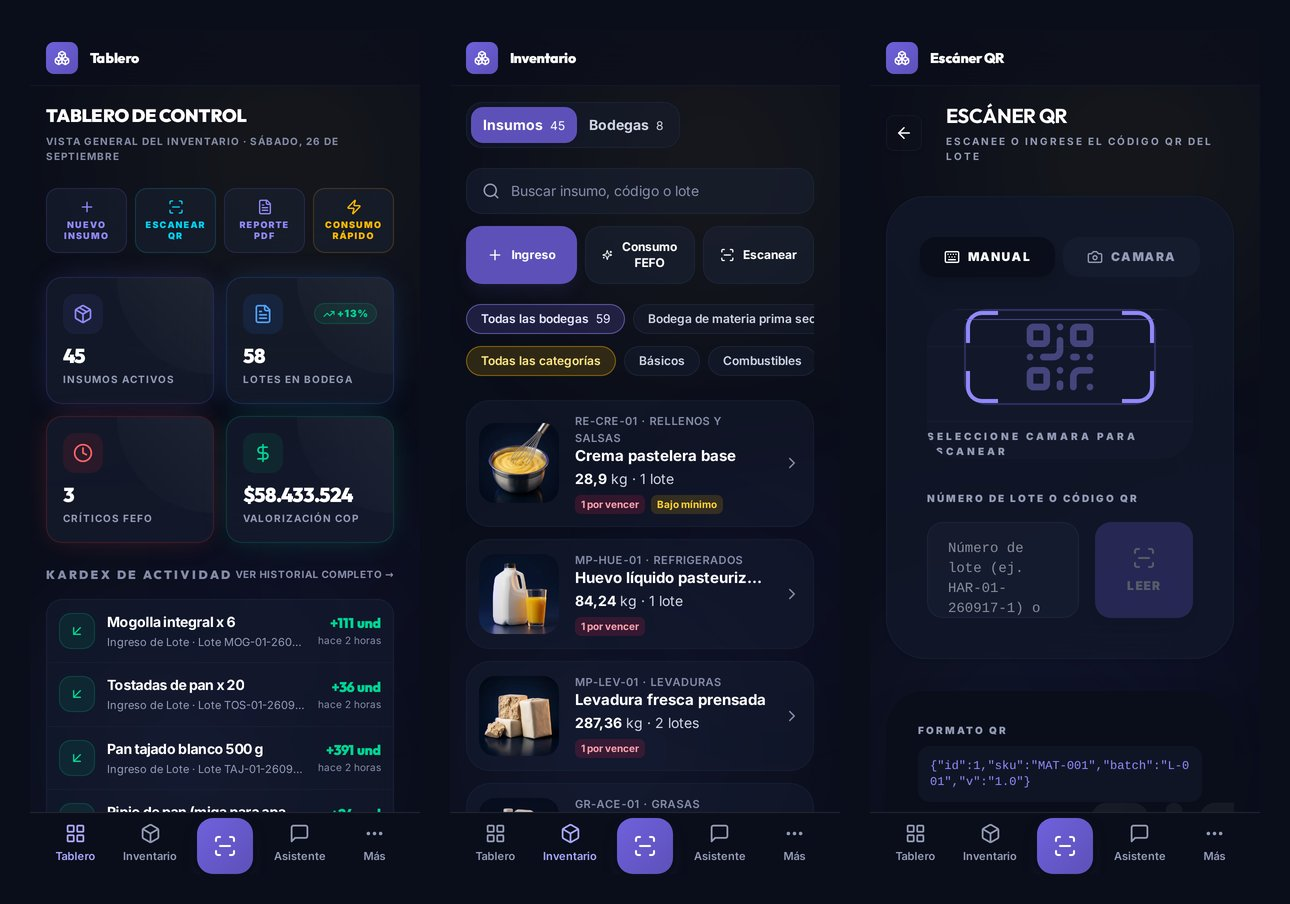
\includegraphics[width=0.8\textwidth]{Anexos/Imagenes/manual/web/14-movil.jpg}\caption{Tablero, inventario y escáner en el celular.}\end{figure}

\end{document}
